%\documentclass{cumcmthesis}
\documentclass[withoutpreface,bwprint]{cumcmthesis} %去掉封面与编号页,电子版提交的时候使用。


\usepackage[framemethod=TikZ]{mdframed}
\usepackage{url}   % 网页链接
\usepackage{subcaption} % 子标题
\usepackage{fancyhdr} 
\usepackage{color}
\usepackage{longtable,booktabs}
\usepackage{setspace}
\usepackage{pythonhighlight}


\title{基于状态转移的自动驾驶电动物料车换电站选址及车辆调度模型}
\tihao{C}
\supervisor{ }
\yearinput{2022}
\monthinput{08}
\dayinput{05}

\begin{document}
	
	\maketitle
	\begin{abstract}
		摘要
		
		
		\quad
		
		
		\keywords{关\quad  键\quad  字\quad }
\end{abstract}

%\begin{spacing}{1.25}
%	\tableofcontents
%\end{spacing}   

\newpage

\setcounter{page}{1}    

\section{问题重述与约束分析}
\subsection{问题重述}



\begin{enumerate}
	\item 
	\item 
	\item 
	\item 
\end{enumerate}



\subsection{约束条件分析}

\begin{itemize}
	\item
	\item 
	\item 
\end{itemize}
 

\section{符号说明与模型假设}
\subsection{符号说明}
本文定义了如表13个使用次数较多的符号, 其余符号在使用时\textbf{注明}




\begin{figure}[!h]
	\centering
	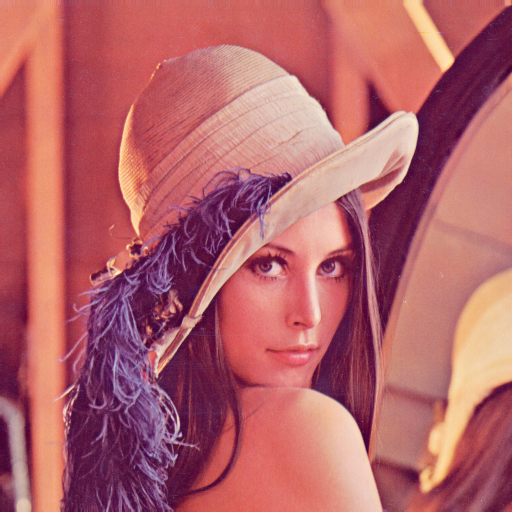
\includegraphics[width=.85\textwidth]{P1}
	\caption{图片示意}
	\label{P1}
\end{figure}


如图\ref{P1}所示,...

\newpage
%参考文献
\begin{thebibliography}{9}%宽度9
	\bibitem[1]{test} 参考文献
\end{thebibliography}



\newpage
%附录
\begin{appendices}
	

	\section{附录}

\begin{python}
import math

def hix(x):
if x > 0:
return 1+1=2
else:
return 0

\end{python}




\end{appendices}





\end{document} 